\chapter{Theory}
In this chapter, an overview of mathematical basic of the soot model is presented, which includes the transport equations, characterization of soot morphology and calculation of source terms corresponding to each step of soot evolution. All equations will be used to implement the soot model in \verb|laminarSoot| library. 
\section{Transport equations}

MPBM relies on the Eulerian description of particles where certain physical properties representative of particle population such as number density, mass or surface area are treated as continuous quantities that can be described by solving scalar transport equations. The formulation of soot model used in this project is based on MPBM originally proposed and validated by Kholghy and Kelesidis \cite{Kholghy2021}, and it tracks number density of primary particles (N\textsubscript{pri}) and agglomerates (N\textsubscript{agg}), total carbon (C\textsubscript{tot}) and hydrogen (H\textsubscript{tot}) content of soot particles by solving the following transport equations

\begin{equation}
	\frac{\partial}{\partial t}(\rho N_{agg}) + \nabla\cdot(\rho u N_{agg})+\nabla^2(\rho D N_{agg}) = \rho\left( S^N_{inc} + S^N_{coag} \right)
	\label{eqn:N_agg},
\end{equation}

\begin{equation}
	\frac{\partial}{\partial t}(\rho N_{pri}) + \nabla\cdot(\rho u N_{pri})+\nabla^2(\rho D N_{pri}) = \rho S^N_{inc}
	\label{eqn:N_pri},
\end{equation}

\begin{equation}
	\frac{\partial}{\partial t}(\rho C_{tot}) + \nabla\cdot(\rho u C_{tot})+\nabla^2(\rho D C_{tot}) = \rho\left( S^C_{inc} + S^C_{grow} + S^C_{ox} \right)
	\label{eqn:C_tot},
\end{equation}

\begin{equation}
	\frac{\partial}{\partial t}(\rho H_{tot}) + \nabla\cdot(\rho u H_{tot})+\nabla^2(\rho D H_{tot}) = \rho\left( S^H_{inc} + S^H_{grow} + S^H_{ox} \right)
	\label{eqn:H_tot}.
\end{equation}

In Equations~\eqref{eqn:N_agg}-\eqref{eqn:H_tot}, S represents the source terms where superscripts indicates the transport equation and subscripts denotes the process the source term is associated with. For example, $\mathrm{S^C_{grow}}$ accounts for the addition of carbon to soot particles via surface growth.

\section{Morphology}
\label{sec:morphology}
Soot particles are formed as agglomerates of spherical primary particles. Incipient soot has spherical shape, and collision and attachment of these spheres results in fractal-like agglomerate. Hereafter, the word \textit{"particle"} refers to soot both in spherical and agglomerate shape.
The morphology of soot agglomerates are characterized by primary particle, mobility, and gyration diameters. These diameters can be related to each other by number of primary particles using power-laws. Mobility and gyration diameters are the diameter of the sphere with the same translational and rotational properties of an agglomerate, respectively. Figure~\ref{fig:Morphology} illustrates the schematics of sample soot agglomerates with 12 primary particles and depicted $\mathrm{d_p}$, $\mathrm{d_m}$, $\mathrm{d_g}$.
\begin{figure}[!htbp]
	\centering
	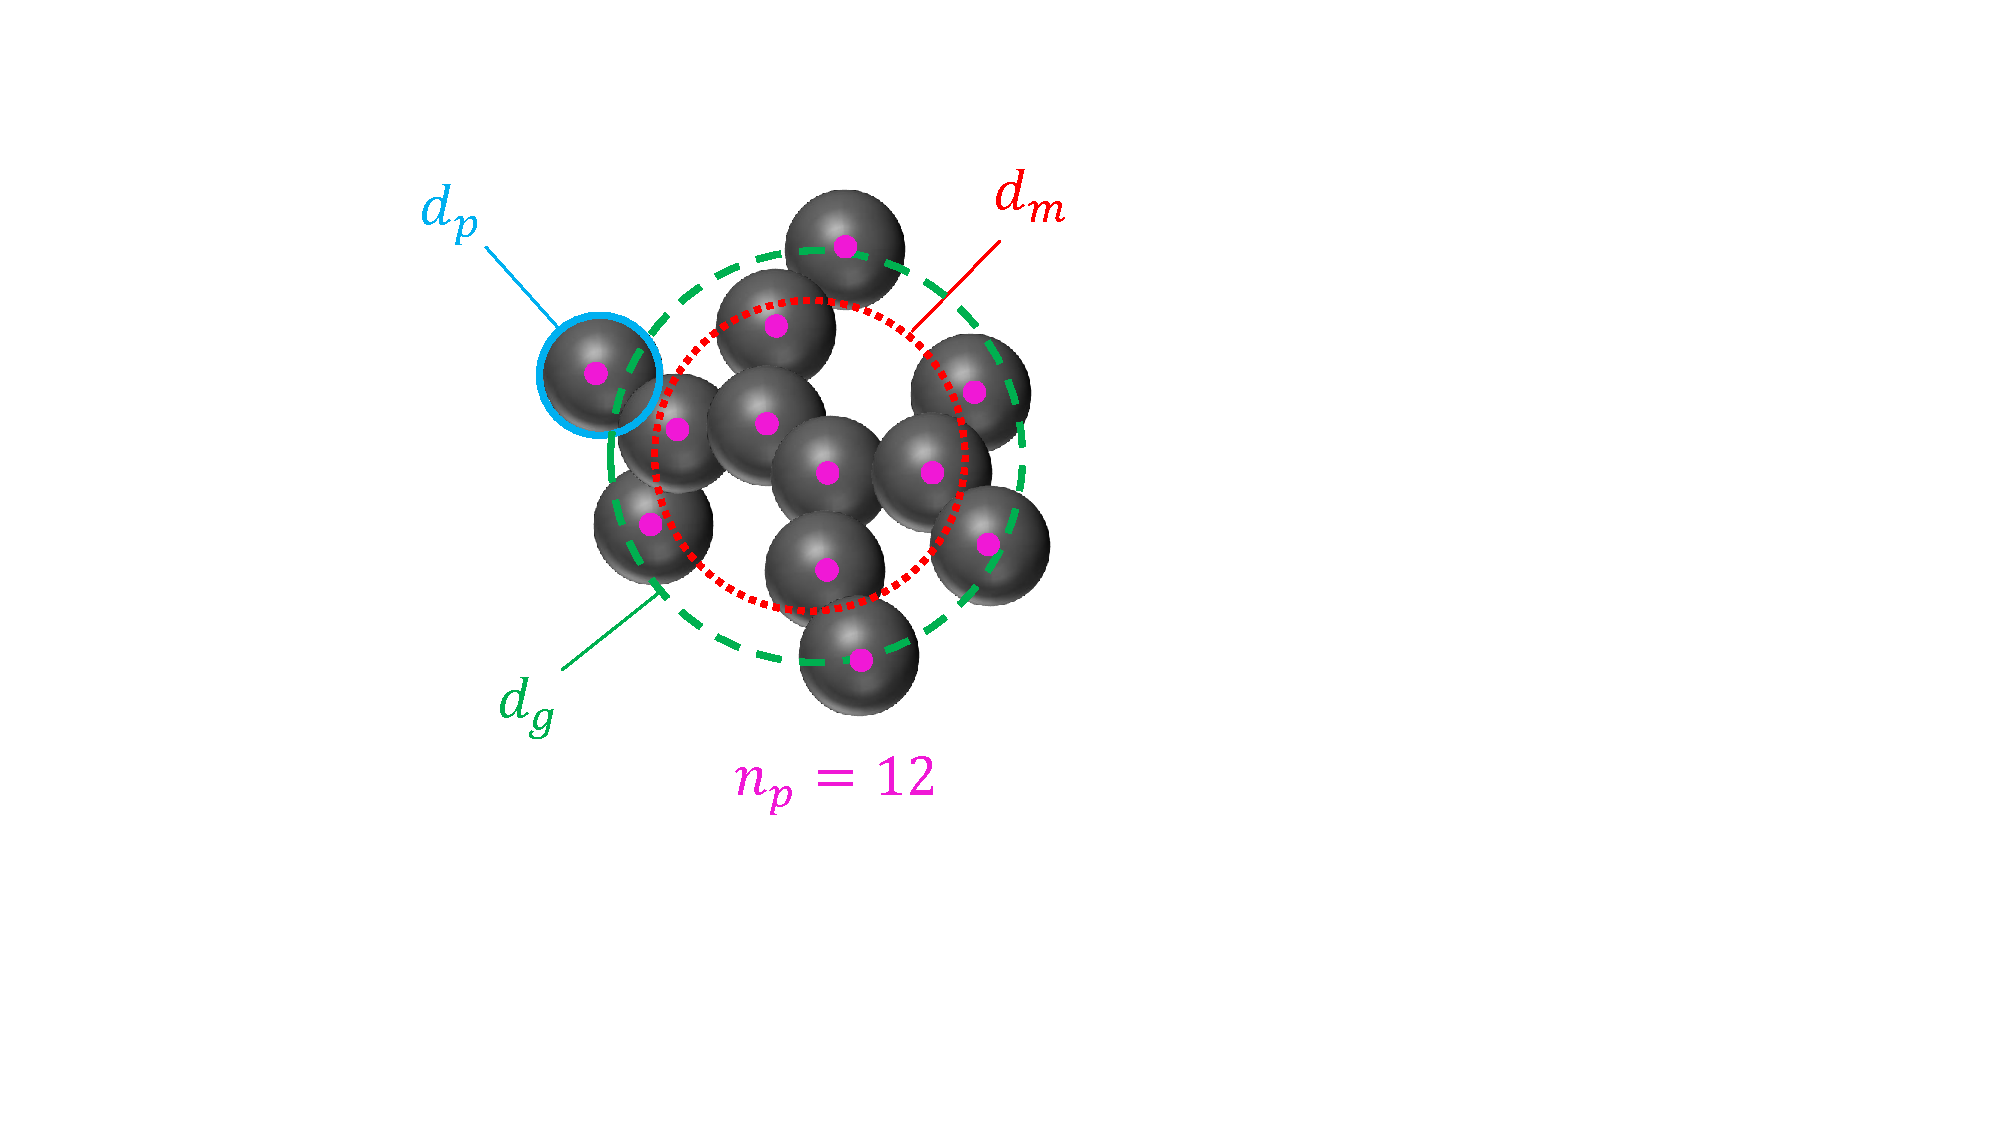
\includegraphics[height=60mm, ]{Figures/Morphology.pdf}
	\caption{The schematics of a soot agglomerates with 12 primary particles ($\mathrm{n_p=12}$). Primary particle ($\mathrm{d_p}$), mobility ($\mathrm{d_m}$), and gyration ($\mathrm{d_g}$) are shown.}
	\label{fig:Morphology}
\end{figure} 

$\mathrm{n_p}$ is the number of primary particles in each agglomerate that can be obtained by dividing the number density of primary particles by that of agglomerates,

\begin{equation}
	n_p = \frac{N_{pri}}{N_{agg}}
	\label{eqn:n_p}.
\end{equation}

Primary particle diameter, $\mathrm{d_p}$, can be obtained from total carbon and number density of primary particles using

\begin{equation}
	d_p = \left(\frac{6}{\pi} \frac{C_{tot}\cdot W_{carbon}}{\rho_{soot}} \frac{1}{N_{pri}\cdot Av} \right)^{1/3}
	\label{eqn:d_p}.
\end{equation}

The DEM-derived power-laws relate $\mathrm{d_m}$ and $\mathrm{d_g}$ to $d_p$ and $\mathrm{n_p}$ as

\begin{equation}
	d_{m} = d_p\cdot n_p^{0.45}
	\label{eqn:d_m},
\end{equation}

\begin{equation}
	d_g = 
	\left\{
	\begin{array}{lr}
		d_m/(n_p^{-0.2}+0.4), & \text{if } n_p > 1.5\\
		d_m/1.29. & \text{if } n_p\leq 1.5
	\end{array}
	\right.
	\label{eqn:d_g}
\end{equation}

$\mathrm{d_{m}}$ and $\mathrm{d_{g}}$ are used to calculate the collision and attachment rate of soot agglomerates that accounts for the coagulation source term.   

\section{Diffusion of soot particles}

The diffusion coefficient of soot particle, $D$, used in Equations~\eqref{eqn:N_agg}-\eqref{eqn:H_tot} is calculated as

\begin{equation}
	D = \frac{k_B T}{f}
	\label{eqn:diff},
\end{equation}
\noindent where $f$ is the friction factor of particles in gas, and it is calculated for free molecular to continuum regimes as

\begin{equation}
	f = \frac{3\pi\mu d_m}{C}
	\label{eqn:fraction},
\end{equation}

\begin{equation}
	C = 1+\frac{2\lambda}{d_m}
	\left(
	1.21+0.4exp(\frac{-0.78d_m}{\lambda})
	\right)
	\label{eqn:cun},
\end{equation}
\noindent where $\lambda$ is the mean free path of gas given as:
\begin{equation}
	\lambda = \frac{\mu}{\rho}\sqrt{\frac{\pi W_{gas}}{2k_B Av T}}
	\label{eqn:lambda}.
\end{equation}


\section{Coagulation}
Coagulation is the process during which solid and hard soot particles collide and attach at point of contact leading to larger agglomerates. This process conserves the soot mass and composition and number density of primary particles, so coagulation only affects $\mathrm{N_{agg}}$ (Equation~\eqref{eqn:N_agg}). $\mathrm{S^N_{coag}}$ accounts for the decay rate of $\mathrm{N_{agg}}$ by the binary collision of soot particles by
\begin{equation}
	S^N_{coag} = -\frac{1}{2}\beta N^2_{agg}
	\label{eqn:Scoag},
\end{equation}
where $\mathrm{\beta}$ is harmonic mean of collision frequency in the continuum ($\mathrm{\beta_{cont}}$) and free molecular ($\mathrm{\beta_{fm}}$) regimes enhanced by \%82 accounting for the polydispersity of particles using the following relations
\begin{equation}
	\beta = 1.82\frac{\beta_{fm}\beta_{cont}}{\beta_{fm}+\beta_{cont}}
	\label{eqn:beta},
\end{equation}
\begin{equation}
	\beta_{fm} = 4\sqrt{\frac{\pi k_b T}{m_{agg}}} d^2_g
	\label{eqn:betafm},
\end{equation}
\begin{equation}
	\beta_{cont} = 8\frac{k_b T}{3\mu} \left( 1+\frac{2\lambda}{d_m}
	\left[
	1.21 + 0.4e^{-\frac{0.78 d_m}{\lambda}}
	\right]
	\right)
	\label{eqn:betacont}.
\end{equation}


\section{Surface growth via HACA}
Hydrogen abstraction carbon addition (HACA) is a major pathway for soot mass growth where active reaction sites on particles form bonds with acetylene ($\mathrm{C_2H_2}$). HACA mechanism \cite{appel2000kinetic} is described by a set of elementary with a given rates that are listed in Table~\ref{tab:HACA}.
The HACA rate is defined as the absolute rate change of concentration of $\mathrm{C_2H_2}$ via HACA mechanism as

\begin{equation}
	\omega_{c_2h_2} = \alpha k_{f4} [\mathrm{C_2H_2}][\mathrm{C_{soot\mbox{\textdegree}}}]
	\label{eqn:hacaRate},
\end{equation}
\begin{equation}
	\frac{d}{dt}\left[ {\mathrm{C_2H_2}} \right] = -\omega_{c_2h_2}
	\label{eqn:c2h2Rate}.
\end{equation}

In Equation~\eqref{eqn:hacaRate}, $\mathrm{k_{f4}}$ refers to forawrd reaction rate of 4th reaction in reaction 4 in Table~\ref{tab:HACA}. The contribution of HACA to growth source terms  can be computed from HACA rate considering the number of carbon atoms in $\mathrm{C_2H_2}$ and number of arm-chair and zig-zag hydrogenated sites on soot particle~\cite{blanquart2009analyzing} using

\begin{equation}
	S^C_{grow|HACA} = 2\omega_{c_2h_2}/\rho
	\label{eqn:SCgrowHACA},
\end{equation}
\begin{equation}
	S^H_{grow|HACA} = 0.25\omega_{c_2h_2}/\rho
	\label{eqn:SHgrowHACA}.
\end{equation}

In Equation~\eqref{eqn:hacaRate}, $\alpha$ is the surface reactivity of soot defined by an empirical relation as 
\begin{equation}
	\alpha = \tanh 
	\left(
	\frac{12.56 - 0.00563\cdot T}
	{\mbox{log}_{10}
		\left( \frac{\rho_{soot}\frac{\pi}{6}d^3_p \cdot Av}{W_{carbon}} \right) } -1.38+0.00068\cdot T
	\right)
	\label{eqn:alpha}.
\end{equation}

$\mathrm{[C_{soot\mbox{\textdegree}}]}$ is the concentration of dehydrogenated site on soot particle computed by
\begin{equation}
	[\mathrm{C_{soot\mbox{\textdegree}}}] = A_{tot}\frac{\rho}{Av}\chi_{soot\mbox{\textdegree}}
	\label{eqn:csoot0}.
\end{equation}

$A_{tot}$ is the total surface area of soot particles obtained as
\begin{equation}
	A_{tot} = N_{pri}Av\cdot \pi d^2_p
	\label{eqn:Atot},
\end{equation}

$\chi_{soot\mbox{\textdegree}}$ is the number of active reaction sites per unit surface area of particles.
\begin{equation}
	\chi_{soot\mbox{\textdegree}} = 
	\frac
	{k_{f1}[\mathrm{H}]+k_{f2}[\mathrm{OH}]}
	{k_{r1}[\mathrm{H_2}]+k_{r2}[\mathrm{H_2O}]+k_{f3}[\mathrm{H}]+k_{f4}[\mathrm{C_2H_2}]+k_{f5}[\mathrm{O_2}]+k_{f1}[\mathrm{H}]+k_{f2}[\mathrm{OH}]} \chi_{soot_{CH}}
	\label{eqn:chisoot0},
\end{equation}

\noindent where $\chi_{soot_{CH}}=2.3\times 10^{19} m^{-2}$. In Equation~\eqref{eqn:chisoot0}, $k_{r1}$ denotes the reverse rate of the first reaction in Table~\ref{tab:HACA}, and the rest of reaction rates follow the same naming convention.

\begin{table}
	\caption{Rate coefficients for the various surface reactions in Arrhenius form $\mathrm{k=AT^n\cdot e^{-E/RT}}$}
	\label{tab:HACA}
	\centering
	\begin{tabular}{l l l l l l}
		\hline
		No. & Reaction & \hspace{0.1cm} & A~$\mathrm{\left[ \frac{m^3}{mol\cdot s} \right]}$ & n & $\mathrm{\frac{E}{R} [K]}$  \\
		\hline
		1 & \ce{C_{soot-H} + H <--> C_{soot\textdegree} + H_2}  & f & $4.17\times 10^7$ & 0 & 6542.52 \\
		& & r & $3.9\times 10^6$ & 0 & 5535.98 \\
		2 & \ce{C_{soot-H} + OH <--> C_{soot\textdegree} + H_2O} & f & $10^4$ & 0.734 & 719.68\\
		&  & r & 3.68$\times 10^2$ & 1.139 & 8605.94 \\
		3 & \ce{C_{soot\textdegree} + H -> C_{soot} + H_2O} & f & $10^4$ & 0.734 & 719.68\\
		4 & \ce{C_{soot\textdegree} + C_2H_2 -> C_{soot-H}} & f & 80 & 1.56 & 1912.43\\
		5 & \ce{C_{soot\textdegree} + O_2 -> 2CO} & f & 2.2 $\times 10^6$ & 0 & 3774.53\\
		6 & \ce{C_{soot}-H + OH -> CO + \frac{1}{2} H_2} & f & 0.13 & 0 & 0\\
		\hline
	\end{tabular}
\end{table}

\section{Oxidation via HACA}
The carbons on the surface of soot are oxidized via reaction with $\mathrm{O_2}$ and $\mathrm{OH}$ which decreases total carbon of soot and releases CO and $\mathrm{H_2}$ to gas mixture. The oxidation process is described by HACA mechanism. $\mathrm{O_2}$ and $\mathrm{OH}$ oxidation rates are calculated as

\begin{equation}
	\omega_{o2} = \alpha k_{f5} [\mathrm{O_2}][C_{soot\mbox{\textdegree}}]
	\label{eqn:hacaO2Rate},
\end{equation}

\begin{equation}
	\omega_{oh} = \alpha k_{f6} [\mathrm{OH}]N_{agg} \rho
	\label{eqn:hacaOHRate}.
\end{equation}

The oxidation source term is calculated considering the number of carbon atoms removed from soot through each oxidation pathway by

\begin{equation}
	S^C_{ox} = -(2\omega_{o2}+\omega_{oh})/\rho
	\label{eqn:SCOx},
\end{equation}

\section{PAH growth models}
\subsection{Reactive Dimerization}

\subsection{Inception}

The inception is described using reactive dimerization of polycylic aromatic hydrocarbons (PAHs) \cite{kholghy2018reactive} where collision of two PAH molecules form physically-bonded dimers followed by their carbonization that results in new soot particles. This two step process can be described as

\begin{equation}
	\ce{PAH_i + PAH_j <-->[k_{FWD}][k_{REV}] Dimer^*_{ij} }
	\label{eqn:phydimer},
\end{equation}
\begin{equation}
	\ce{Dimer^*_{ij} ->[k_{REAC}] Dimer_{ij} }
	\label{eqn:chemdimer}.
\end{equation}

In Equation~\eqref{eqn:phydimer}, $k_{FWD}$ is the forward rate of physical dimerization and computed as

\begin{equation}
	k_{FWD} = 2.2 \cdot 0.1 \cdot Av\cdot d^2_{ij} \sqrt{\frac{8\pi k_B T}{m_{ij}}}
	\label{eqn:kFWD},
\end{equation}

\noindent where $d_{ij}=2d_id_j/(d_i+d_j)$ and $m_{ij}=m_im_j/(m_i+m_j)$ are reduced diameter and mass of PAH molecules in the dimer, respectively. The mass of PAH is calculated by dividing the molecular weight by Avogadro's number. The diameter is estimated by assuming a sphere with the mass of one PAH molecule and an estimated density \cite{johansson2017evolution} using 

\begin{equation}
	m_{PAH} = \frac{W_{PAH}}{Av}
	\label{eqn:PAHmass},
\end{equation}

\begin{equation}
	\rho_{PAH} = 
	171943.5197\frac{n_{C,PAH}W_{carbon}+n_{H,PAH}W_{hydrogen}}{n_{C,PAH}+n_{H,PAH}}
	\label{eqn:PAHrho},
\end{equation}

\begin{equation}
	V_{PAH} =
	\frac{m_{PAH}}{\rho_{PAH}}
	\label{eqn:PAHvolume},
\end{equation}

\begin{equation}
	d_{PAH} = 
	\left(
	\frac{6V_{PAH}}{\pi}
	\right)^{1/3}
	\label{eqn:PAHdiameter}.
\end{equation}


The reverse rate of physical dimerization, $\mathrm{k_{REV}}$, is calculated from $\mathrm{k_{FWD}}$ and equilibrium coefficient of physical dimerization as

\begin{equation}
	k_{REV} = k_{FWD}10^{-b}e^{-a\epsilon ln(10)/(RT)}
	\label{eqn:kREV},
\end{equation}
\begin{equation}
	\epsilon = cW_{ij} -d
	\label{eqn:epsilon},
\end{equation}
\noindent where $W_{ij}=W_iW_j/(W_i+W_j)$ is the reduced molecular mass of dimer, $\mathrm{a=0.115}$ (obtained from pyrere dimerization data~\cite{sabbah2010exploring}) and b=1.8 \cite{kholghy2018reactive}, c=933420~j/kg, and d=34053~j/mol~\cite{kholghy2018reactive}. 

The rate of chemical bond formation, $\mathrm{k_{REAC}}$ is defined in the Arrhenius form~\cite{naseri2022simulating} as
\begin{equation}
	k_{REAC} = 5\times10^6\cdot e^{(-96232/RT)}
	\label{eqn:kREAC}.
\end{equation}

Assuming a steady state condition for the physical dimers, $\mathrm{\partial [Dimer^*_{ij}]/\partial t=0}$, the formation of dimer can be obtained as

\begin{equation}
	\omega_{dimer_{ij}} = k_{REAC}\frac{k_{FWD}[PAH_i][PAH_j]}{k_{REV}+k_{REAC}}
	\label{eqn:ropdimer}.
\end{equation}

The PAHs forming the dimer is removed from the gas mixture due to inception at the same rate as dimerization meaning that

\begin{equation}
	\omega_{PAH_{i}} = \omega_{PAH_{j}} = - \omega_{dimer_{ij}}
	\label{eqn:ropdimer}.
\end{equation}

Here, we assume the smallest soot particle are 2nm in diameter corresponding to a spherical particle with 378 carbon and 20 hydrogen atoms, respectively. The contribution of each dimer to number density (both agglomerates and primary particles), carbon and hydrogen content of particles is proportional to the mass, number of carbon and hydrogen atoms of that dimer, respectively, which is described by

\begin{equation}
	S^N_{inc} = \sum_{i=1}^{n} \sum_{j=i}^{n} \frac{C_{ij}}{C_{min}} \omega_{dimer_{ij}}
	\label{eqn:SNinc},
\end{equation}

\begin{equation}
	S^C_{inc} = \sum_{i=1}^{n} \sum_{j=i}^{n} C_{ij} \omega_{dimer_{ij}}
	\label{eqn:SCinc},
\end{equation}

\begin{equation}
	S^H_{inc} = \sum_{i=1}^{n} \sum_{j=i}^{n} H_{ij} \omega_{dimer_{ij}}
	\label{eqn:SHinc},
\end{equation}
\noindent where $\mathrm{C_{ij}}$ and $\mathrm{H_{ij}}$ are number of carbon and hydrogen atoms in $\mathrm{dimer_{ij}}$, respectively. n is the number of PAHs designated as soot precursors.
Note that, Equation~\eqref{eqn:SNinc} approximates the mass of soot as mass of carbon atoms comprising the particle.

\subsection{Surface growth via PAH adsorption}
The adsorption of PAHs on the surface is a major mass growth pathway of soot particles. Here, a two-step process, similar to inception, is used to address the PAH adsorption. The collision of PAH molecule leads to physically bonded, $\mathrm{Soot-PAH^*}$, that is followed by chemical bond formation, and completes the adsorption process. The following reactions describes the process

\begin{equation}
	\ce{PAH + Soot <-->[k_{fw,ad}][k_{rv,ad}] Soot-PAH^*}
	\label{eqn:phyad},
\end{equation}

\begin{equation}
	\ce{Soot-PAH^* ->[k_{rc,ad}] Soot-PAH}
	\label{eqn:chemad}.
\end{equation}

The forward rate of physical adsorption, $\mathrm{k_{fw,ad}}$, in Equation~\eqref{eqn:phyad} is computed by harmonic mean of collision frequency of soot particles and PAH molecules in free molecular and continuum regime as

\begin{equation}
	k_{fw,ad} = \frac{\beta_{fm,ad}\cdot\beta_{cont,ad}}{\beta_{fm,ad}+\beta_{cont,ad}} Av
	\label{eqn:phyad},
\end{equation}

\noindent where $\beta_{fm,ad}$ is obtained \cite{naseri2022simulating} as

\begin{equation}
	\beta_{fm,ad} = 2.2 
	\sqrt
	{
		\frac{\pi k_B T}{2}
		\left(
		\frac{1}{m_{agg}}+\frac{1}{m_{PAH}} 
		\right)
	} 
	\left( d_g + d_{PAH} \right)^2
	\label{eqn:betafmad},
\end{equation}
\noindent where $m_{agg}=C_{tot}\cdot W_{carbon}/(N_{agg}\cdot Av)$ is the mass of soot agglomerate. $\beta_{cont,ad}$ is computed by

\begin{equation}
	\beta_{cont,ad} =
	\frac{2k_BT}{3 \mu}
	\left[
	\frac{C_s(d_m)}{d_g}
	+
	\frac{C_s(d_{PAH})}{d_{PAH}}
	\right]
	\left( d_g + d_{PAH} \right)
	\label{eqn:betacontad},
\end{equation}

\begin{equation}
	C_s(d) =
	1+
	\frac{2\lambda}{d}
	\left[
	1.21 + 0.4 e^{(-0.78d/\lambda)}
	\right]
	\left( d_g + d_{PAH} \right)
	\label{eqn:cs}.
\end{equation}

The reverse rate of physical adsorption, $\mathrm{k_{rv,ad}}$, is computed similar to reverse physical inception rate (Equation~\eqref{eqn:kREV}) as

\begin{equation}
	k_{rv,ad} = k_{fw,ad}10^{-b}e^{-a\epsilon ln(10)/(RT)}
	\label{eqn:krvad},
\end{equation}
\begin{equation}
	\epsilon = c\frac{MW_{soot}\cdot MW_{PAH}}{MW_{soot} + MW_{PAH}} -d
	\label{eqn:epsilonad},
\end{equation}

\noindent where $\mathrm{MW_{soot}=C_{tot}\cdot W_{carbon} / N_{agg}}$ is the equivalent molecular weight of soot, and a, b, c, and d have the same values as Equation~\eqref{eqn:kREV}.

The rate of chemical adsorption, $\mathrm{k_{rc,ad}}$ is defined in the Arrhenius form~\cite{naseri2022simulating} as
\begin{equation}
	k_{rc,ad} = 2\times10^{10}\cdot e^{(-96232/RT)}
	\label{eqn:krcad}.
\end{equation}

The total adsorption rate can be calculated assuming a steady-state concentration for physically adsorbed PAH on soot, $\mathrm{\partial{[{Soot-PAH^*}]}/\partial t = 0}$, similar to inception rate (Equation~\eqref{eqn:ropdimer}) as\\

\begin{equation}
	\omega_{pah,ad} = k_{rc,ad}\frac{k_{fw,ad}[Soot][PAH]}{k_{rv,ad}+k_{rc,ad}}
	\label{eqn:road},
\end{equation}

\begin{equation}
	[Soot] = \rho N_{agg}
	\label{eqn:sootconcen}.
\end{equation}


The contribution of PAH adsorption rate to particle carbon and hydrogen content is computed as

\begin{equation}
	S^C_{grow|ad} =
	\sum_{i=1}^{n} 
	C_{PAH,i}\cdot\omega_{pah,ad,i}
	\label{eqn:SCad},
\end{equation}

\begin{equation}
	S^H_{grow|ad} =
	\sum_{i=1}^{n} 
	(H_{PAH,i}-2)\cdot\omega_{pah,ad,i}
	\label{eqn:SHad}.
\end{equation}

The rate of removal of PAH from gas mixture due to adsorption is given as

\begin{equation}
	\omega_{PAH,i} =
	-\omega_{pah,ad,i}
	\label{eqn:pahscrubingad}.
\end{equation}

The total growth rate is sum of growth due by HACA and adsorption as

\begin{equation}
	S^C_{grow} =
	S^C_{grow|HACA} + S^C_{grow|ad}
	\label{eqn:SCgrow},
\end{equation}

\begin{equation}
	S^H_{grow} =
	S^H_{grow|HACA} + S^H_{grow|ad}
	\label{eqn:SHgrow}.
\end{equation}


